\chapter{Evaluation}

\section{Prior Information}

This section will evaluate the application of prior information in a setting where a robot hand moves towards and object and back, with two sources of depth data. The two sources of depth information are: enhanced stereo matching using IR dot patterns (denoted as \emph{stereo}) and structured light (denoted as \emph{xtion} as in Asus Xtion).

\subsection{Setup}

A robot is placed in front of a table with an object on it. The left hand is moving from close to the table plane towards the object. Once the object is pushed, the hand moves up and back to its initial position. Figure \ref{fig:bottle_move_trace} shows the trace of the position of the left palm as it moves towards the object and back. The stereo point cloud shows the final state at the end of the movement.
%
\begin{figure}
\centering
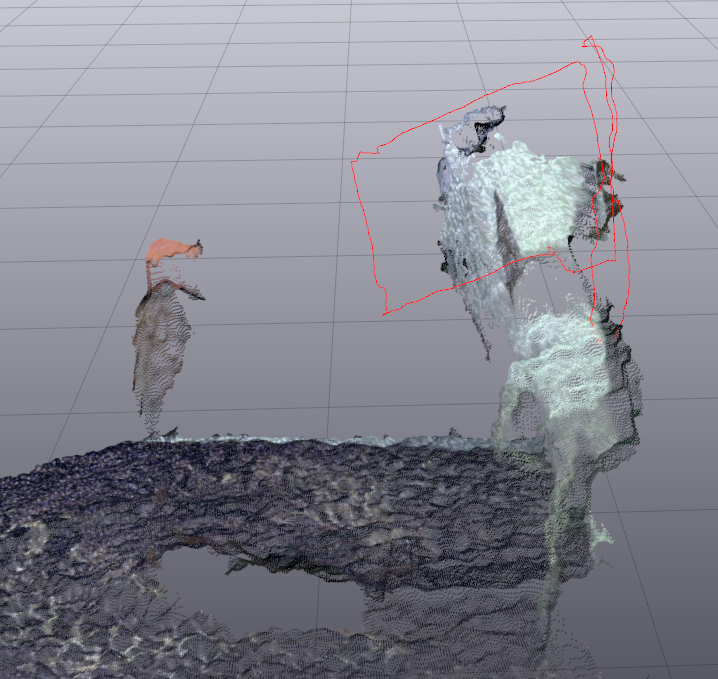
\includegraphics[width=0.5\textwidth]{images/eval_prior/bottle_movement_trace.png}
\caption{Trace of left palm movement. Stereo point cloud shows the final pose.}
\label{fig:bottle_move_trace}
\end{figure}
%
The phases of the movement are defined in table \ref{tab:movement_phases}.

\begin{table}
\centering
\begin{tabular}{|c|l|l|}
\hline
 & \emph{time (s)} & \emph{movement description} \\
\hline
1 & 0...5 & upward \\
\hline
2 & 5...10 & downward \\
\hline
3 & 10...20 & towards object \\
\hline
4 & 20...30 & upward away from object \\
\hline
5 & 30...35 & downward \\
\hline
\end{tabular}
\caption{Phases of arm movement}
\label{tab:movement_phases}
\end{table}

During the movement, depth data is collected simultaneously from the MultiSense stereo sensor and the Asus Xtion structured light sensor. Hence, the stereo feature matching benefits from the distinctive IR dots.

\subsection{Hypotheses}

The deviation of the estimated to the reported robot state is measured in joint and task space. Hence, the error is defined as measurements of the reported pose minus measurements of the estimated pose.

\begin{itemize}
\item deviation to reported pose decreases with increasing weight
\item distraction from surrounding points from objects
\end{itemize}

\subsection{Results}

The error in joint and task space is computed as L2 norm (Euclidean distance) of its components and plotted over time. In joint space these components are the left fingers (13 DoF: 3 \emph{leftIndexFingerPitch}, 3 \emph{leftMiddleFingerPitch}, 3 \emph{leftPinkyPitch}, 3 \emph{leftThumbPitch} and 1 \emph{leftThumbRoll}) and the left arm (7 DoF: \emph{leftShoulderPitch/Roll/Yaw}, \emph{leftElbowPitch}, \emph{leftForearmYaw}, \emph{leftWristRoll/Pitch}). In task space, the 6DoF pose of the left hand (frame: \emph{leftPalm}) is computed via FK on the reported and estimated robot configuration. The position and orientation error are individually plotted.

\subsubsection{Common Weight}

The plots compare the joint and task space errors for the two depth sources for common weights in the range 0 to 5. The common weighting scheme \emph{Weighted L2 norm of joint position deviation} (equation \ref{eqn:objf_weightedL2}) is applied. A weight of 0 indicates that no prior is used at all.

\paragraph{Stereo}

Figure \ref{fig:stereo_joint_error} compares the joint error for left fingers and arm. For both parts, after the optimization reaches the steady state, the maximum error is reached when no prior information from the reported configuration is used.
The general trend is that the error decreases with increasing weight. This is not true for the arm movement in the second half of phase 4, where weights of $0.2$ and $0.5$ result in larger errors than using no prior.

The largest decrease in error can be seen for the finger joints when using already a small weight of $0.2$. A similar effect is not present for the arm joints. This is presumably because the robot can only observe the lower part of its arm and hence the arm configuration is mostly determined by its initial state close to the reported state.


\begin{figure}
\centering
\subfloat[finger joints]{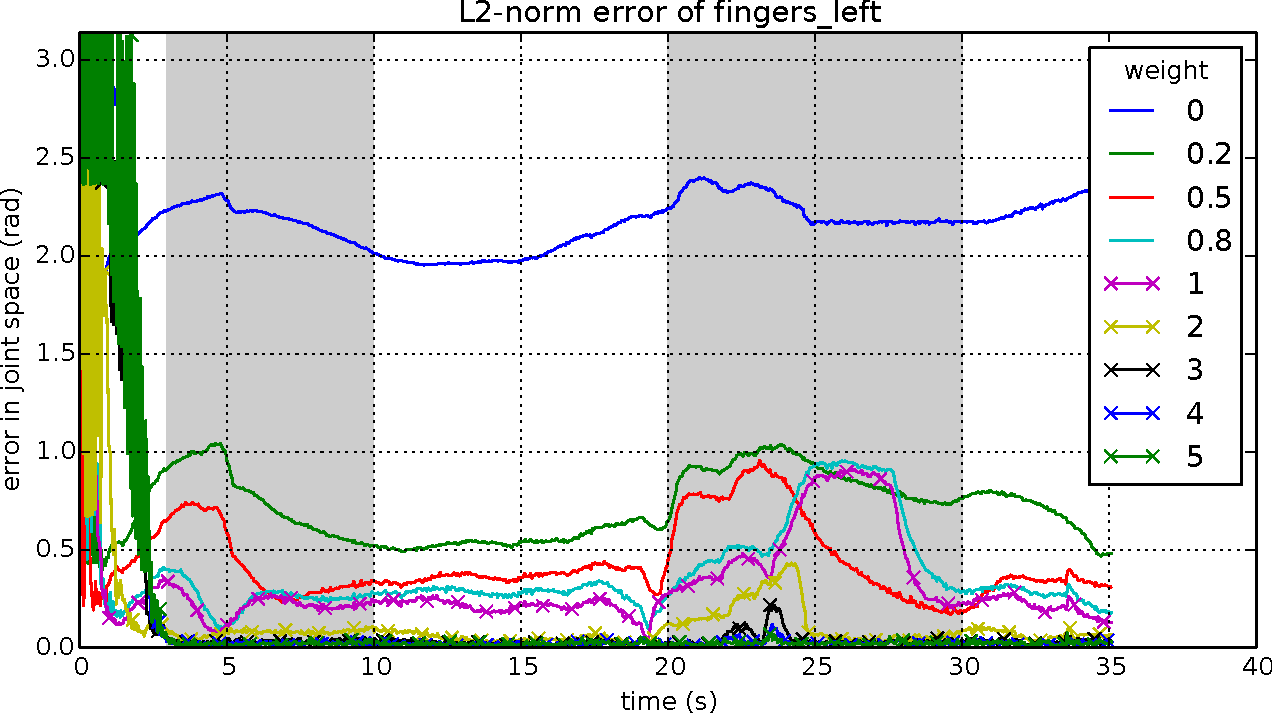
\includegraphics[width=0.5\textwidth]{images/eval_prior/common_weights/stereo_finger_joint_error.pdf} \label{fig:stereo_joint_error_hand} }
%
\subfloat[arm joints]{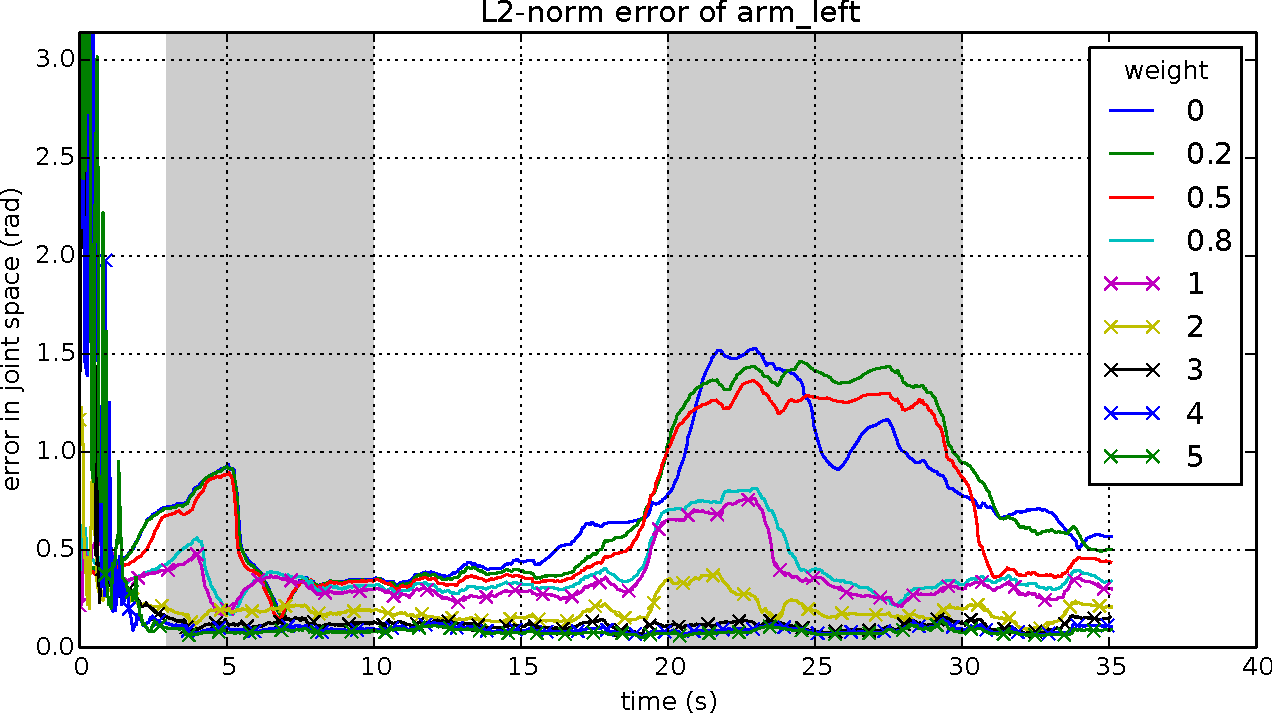
\includegraphics[width=0.5\textwidth]{images/eval_prior/common_weights/stereo_arm_joint_error.pdf} \label{fig:stereo_joint_error_arm} }
\caption{Stereo, joint space error for left finger and arm joints}
\label{fig:stereo_joint_error}
\end{figure}

As the hand position and orientation only depends on the arm configuration but not the finger configuration, we expect some relation between the joint error of the arm and the pose error on the hand frame. We can see this relation, when comparing the joint space error for the arm in figure \ref{fig:stereo_joint_error_arm} and the hand pose error in figure \ref{fig:stereo_hand_pose_error}. In particular the error increases in phases where the hand moves upwards and when it moves away from the object. The position error can be reduced significantly when using a prior with low weight ($0.2$), where as the orientation error reduces only when using prior weights larger or equal than $0.8$.

\begin{figure}
\centering
\subfloat[position error]{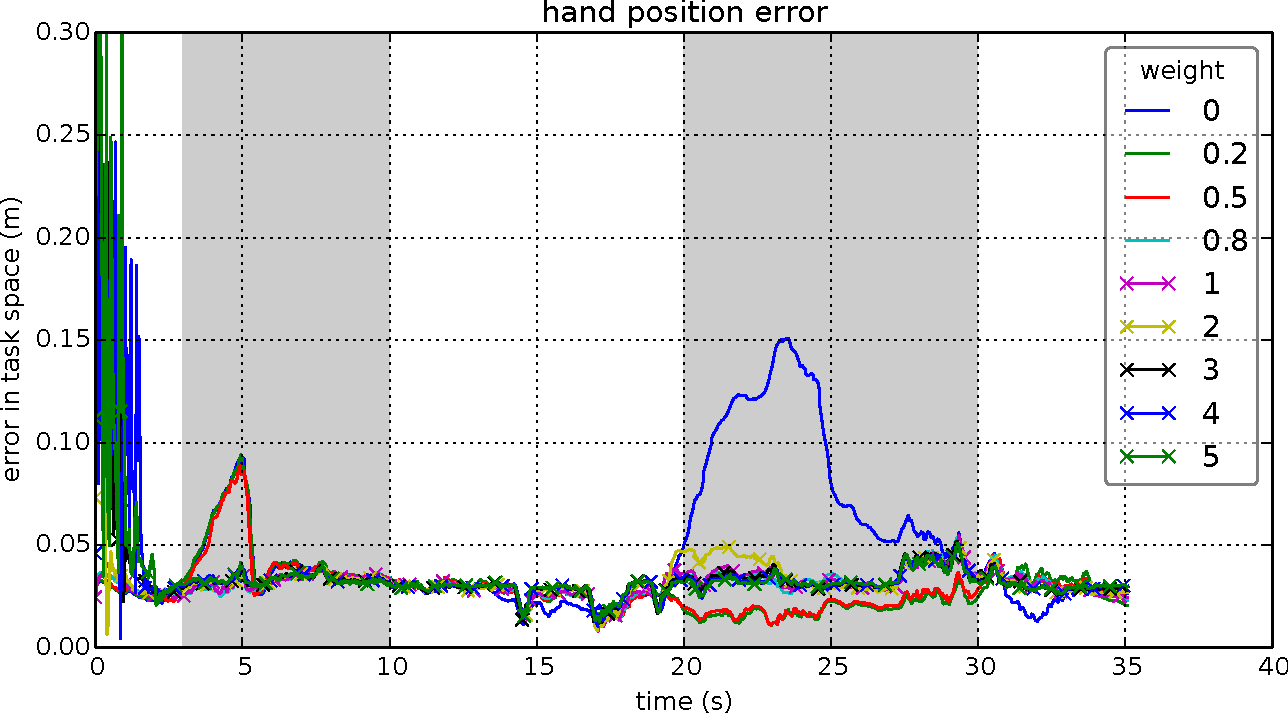
\includegraphics[width=0.5\textwidth]{images/eval_prior/common_weights/stereo_hand_pos_error.pdf} \label{fig:stereo_hand_pos_error}}
%
\subfloat[orientation error]{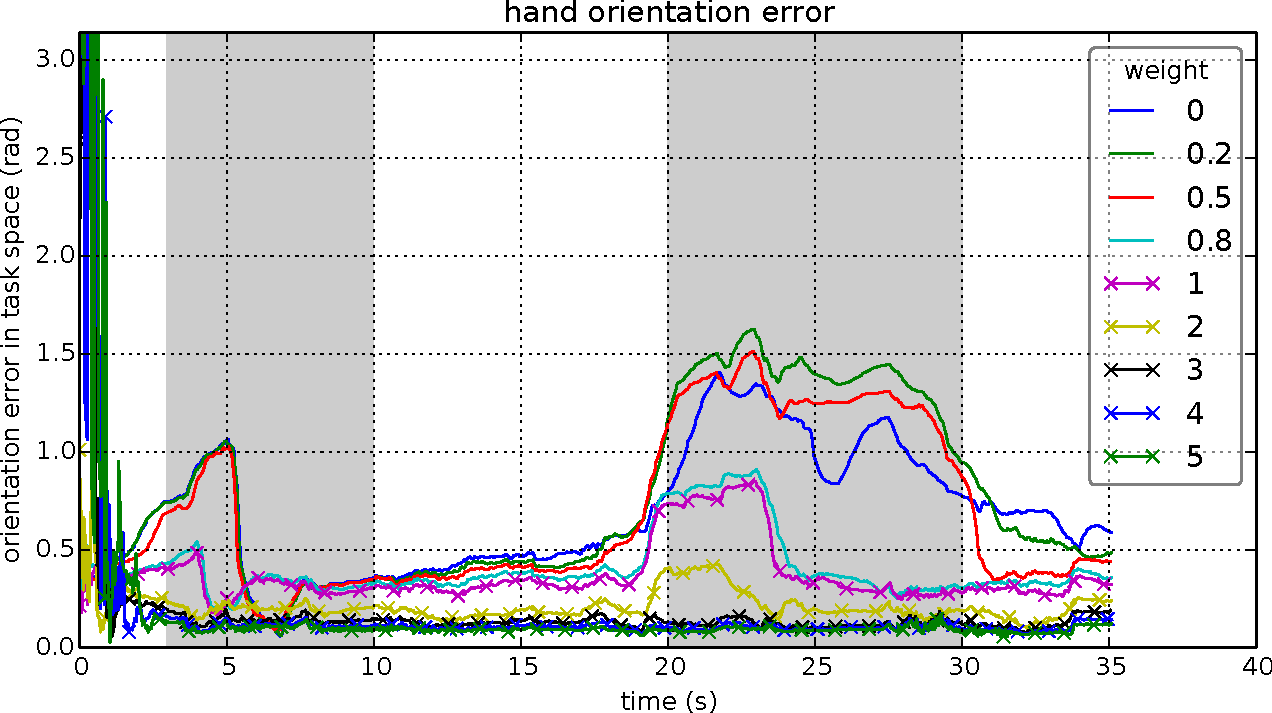
\includegraphics[width=0.5\textwidth]{images/eval_prior/common_weights/stereo_hand_ori_error.pdf}
\label{fig:stereo_hand_ori_error}}
\caption{Stereo, task space error for left hand pose}
\label{fig:stereo_hand_pose_error}
\end{figure}



\paragraph{Asus Xtion}

Using the structured light sensor Asus Xtion, the behaviour of decreasing error with increasing weight is comparable to that one saw for the stereo matching sensor. Similar to the stereo sensor (figure \ref{fig:stereo_joint_error_hand}), the error on the finger joints reduces significantly when already using a small weight of $0.2$ (figure \ref{fig:xtion_joint_error_hand}).
In contrast to small the error on the arm joints when using stereo in the phase of moving towards the object (figure \ref{fig:stereo_joint_error_arm}), the error in this phase when using the Xtion sensor is fairly large for no and low weighted prior (figure \ref{fig:xtion_joint_error_arm}).

\begin{figure}
\centering
\subfloat[finger joints]{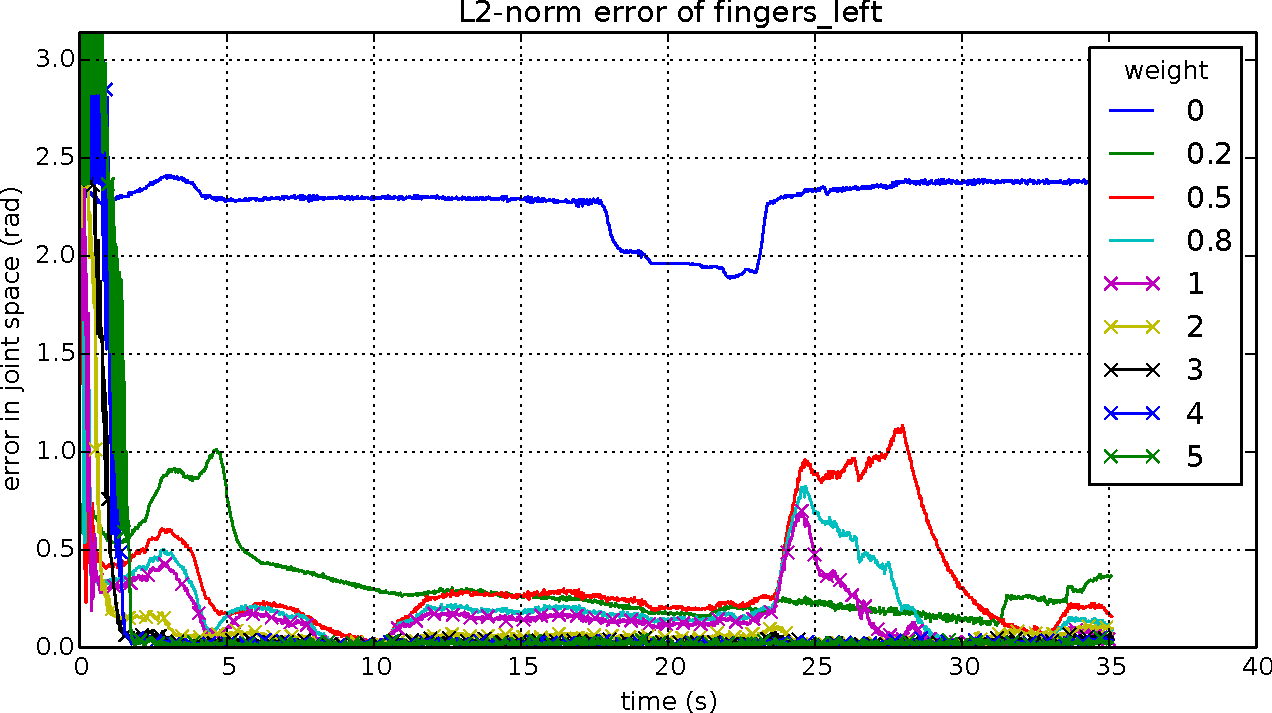
\includegraphics[width=0.5\textwidth]{images/eval_prior/common_weights/xtion_finger_joint_error.pdf} \label{fig:xtion_joint_error_hand}}
%
\subfloat[arm joints]{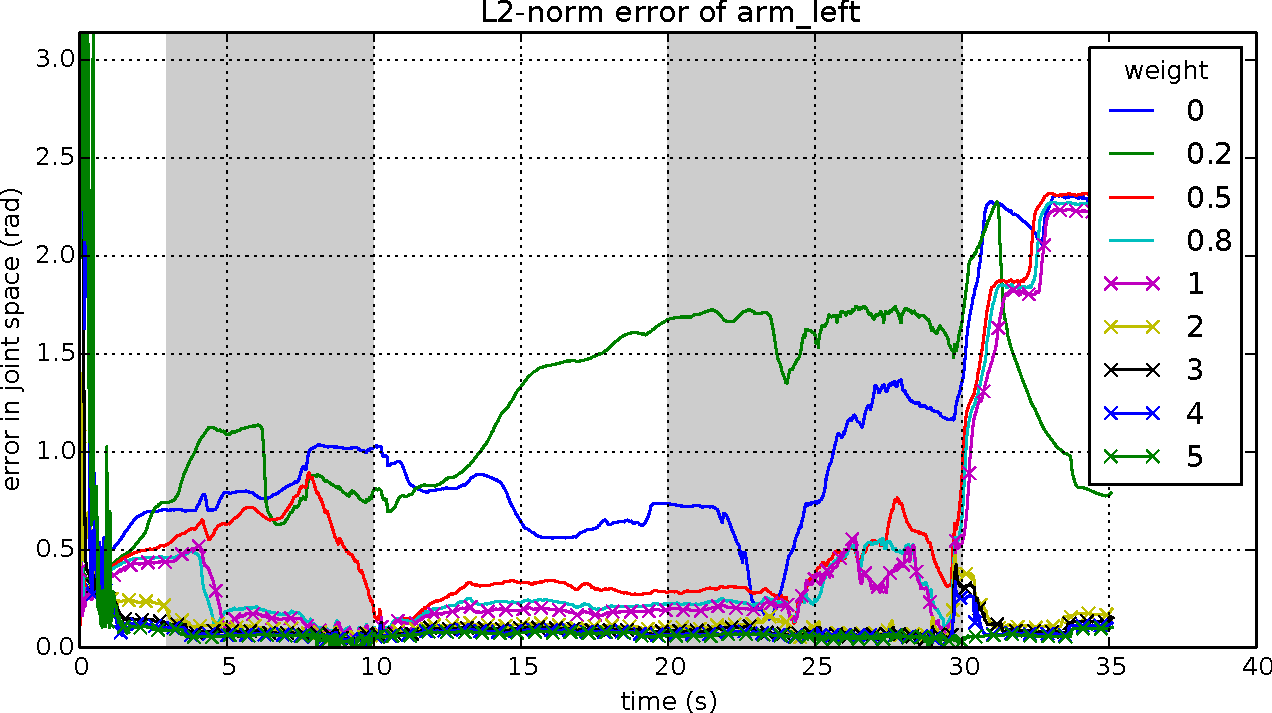
\includegraphics[width=0.5\textwidth]{images/eval_prior/common_weights/xtion_arm_joint_error.pdf} \label{fig:xtion_joint_error_arm}}
\caption{Xtion, joint space error for left finger and arm joints}
\label{fig:xtion_joint_error}
\end{figure}

As before, the hand pose error is only effected by the arm joint errors and thus the hand position error shown in figure \ref{fig:xtion_hand_pos_error} is large in the same moving phase towards the object. For using the structured light sensor, a common weight of at least $2$ is required to drive the solution towards the reported hand position.

\begin{figure}
\centering
\subfloat[position error]{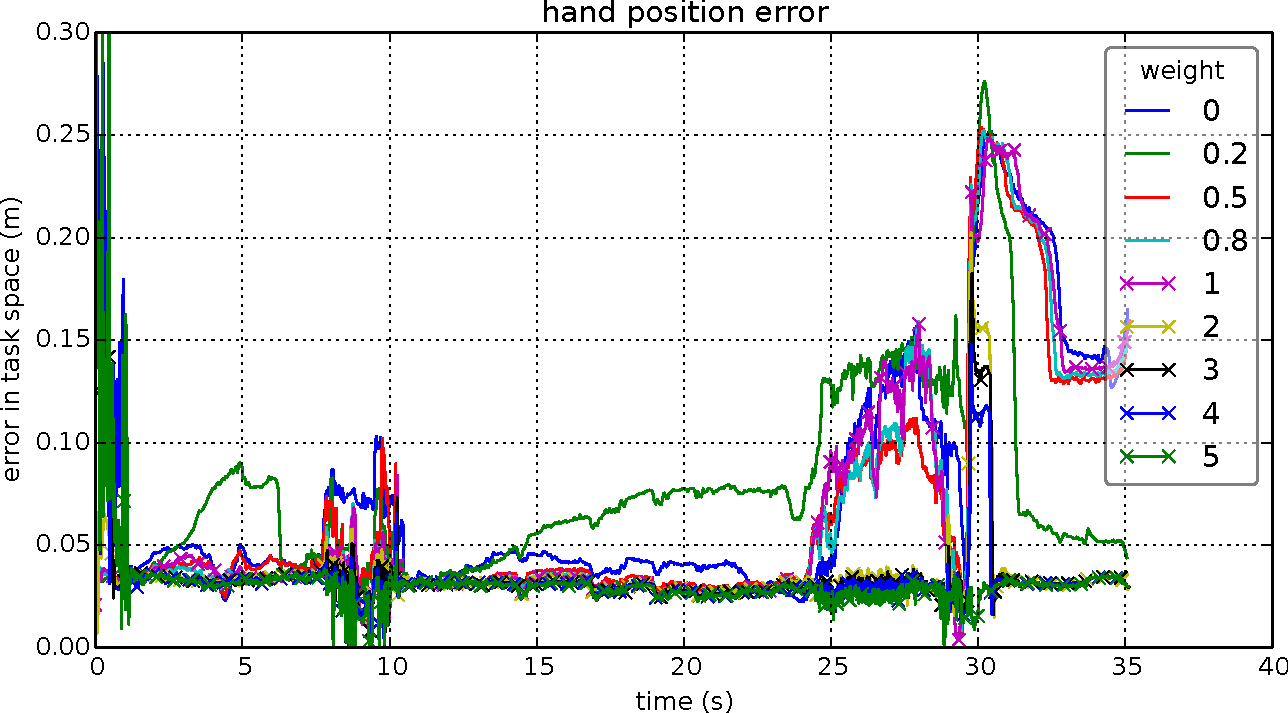
\includegraphics[width=0.5\textwidth]{images/eval_prior/common_weights/xtion_hand_pos_error.pdf} \label{fig:xtion_hand_pos_error}}
%
\subfloat[orientation error]{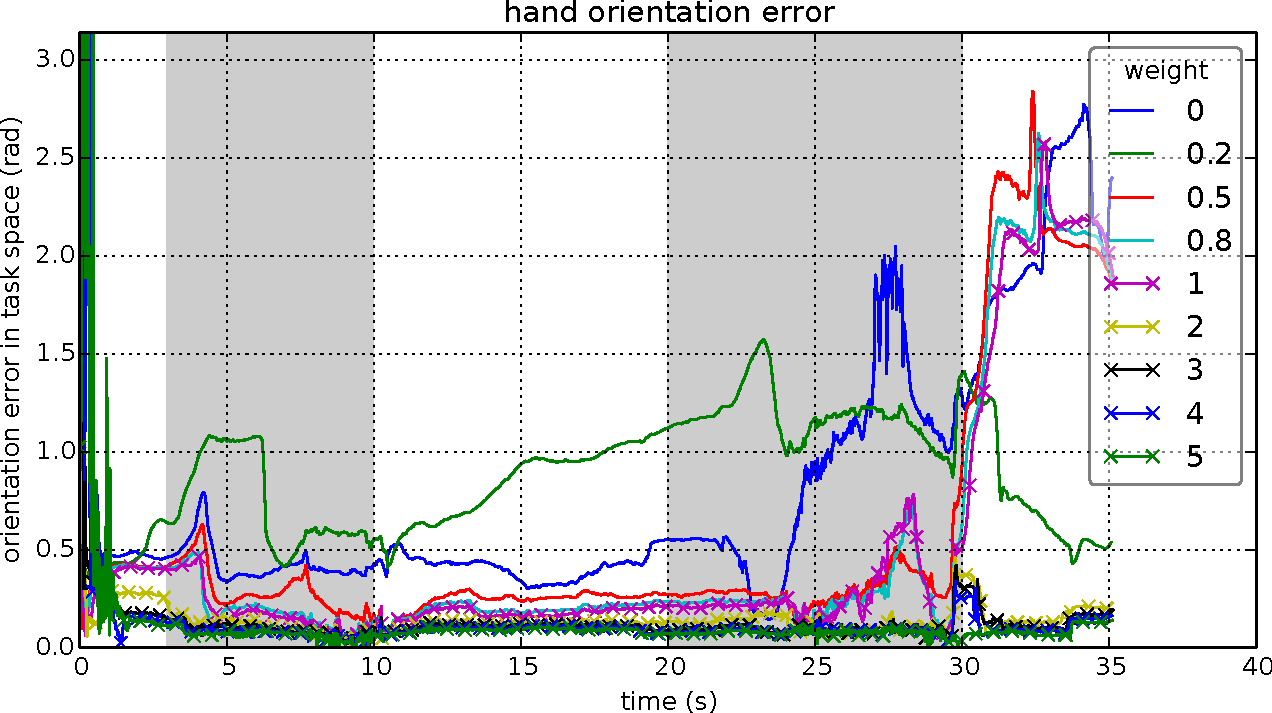
\includegraphics[width=0.5\textwidth]{images/eval_prior/common_weights/xtion_hand_ori_error.pdf} \label{fig:xtion_hand_ori_error}}
\caption{Xtion, task space error for left hand pose}
\label{fig:xtion_hand_pose_error}
\end{figure}

\subsubsection{Individual Weights}

Individual weighting is applied to only stereo depth data. This weighting scheme enables to weight each combination of joint derivations separately as defined by equation \ref{eqn:objf_indiv_weighted}. For simplicity, only single joint deviations are weighted. That is, the weight matrix $Q$ will be a diagonal matrix where only the diagonal elements $q_{i,i}$ will be changed.

In this scenario, three setting of joints are weighted and this scheme is captured in the legend as follows: first, all diagonal elements of $Q$ are set to the weight \emph{q}, second, the 13 finger joints are set to the weight \emph{fingers} and optionally third, the two palm joints (leftWristRoll, leftWristPitch) are set to the value \emph{parm}. E.g., a plot named \texttt{q 1, fingers 0.2, palm 5} indicates that finger joints in the diagonal are weighted by $0.2$, palm joints are weighted with $5$ and the remaining joints are weighted with $1$.

Figure \ref{fig:indiv_joint_error} shows again the joint space error for fingers and arms separately. From these plots we can see that the individual weighting affects the fingers and the arm in different ways. The finger joint error in figure \ref{fig:indiv_joint_error_hand} shows that, raising the palm weights and keeping the remaining constant actually impairs the performance (e.g., compare constant \texttt{q 1, fingers 0.2} and palm weights raised to \texttt{palm 5}). In contrast to this, the arm joint error is reduced when increasing the palm weights and keeping remaining weights constant (e.g., compare constant \texttt{q 0.2, fingers 0.2, palm 5} and palm weights raised to \texttt{q 0.2, fingers 0.2, palm 25}).

\begin{figure}
\centering
\subfloat[finger joints]{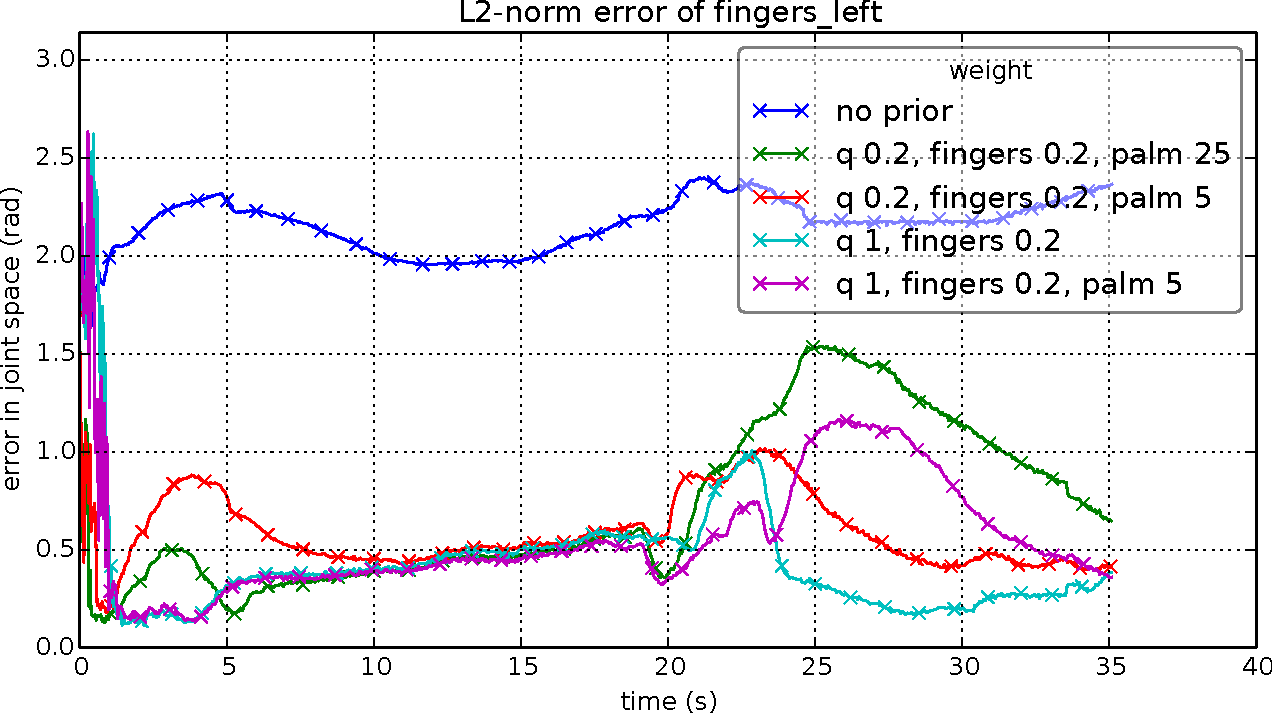
\includegraphics[width=0.5\textwidth]{images/eval_prior/inidv_weights/stereo_finger_joint_error.pdf} \label{fig:indiv_joint_error_hand}}
%
\subfloat[arm joints]{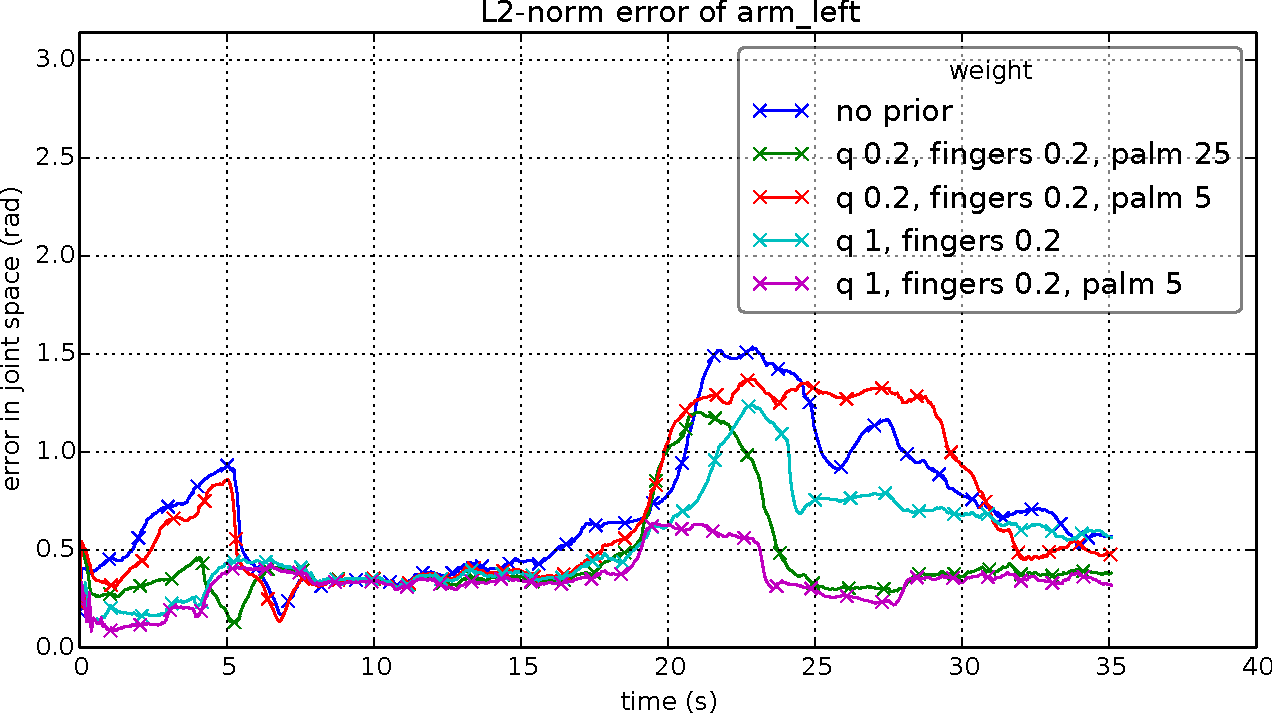
\includegraphics[width=0.5\textwidth]{images/eval_prior/inidv_weights/stereo_arm_joint_error.pdf} \label{fig:indiv_joint_error_arm}}

\caption{Joint space error for individual weighting}
\label{fig:indiv_joint_error}
\end{figure}

Again, the arm joints directly influence the pose error of the hand as seen in figure \ref{fig:indiv_pose_error}. Figure \ref{fig:indiv_hand_pos_error} shows that the hand position mostly benefits from using some prior $>1$ on the palm joints whereas weighting the remaining joints does contribute to driving the solution towards the reported hand position. For the hand orientation error in figure \ref{fig:indiv_hand_ori_error}, the error is usually reduced if the weights on the palm joints are increased (e.g. $1$ to $5$, or $5$ to $25$) and remaining joints keep their weights.

\begin{figure}
\centering
\subfloat[]{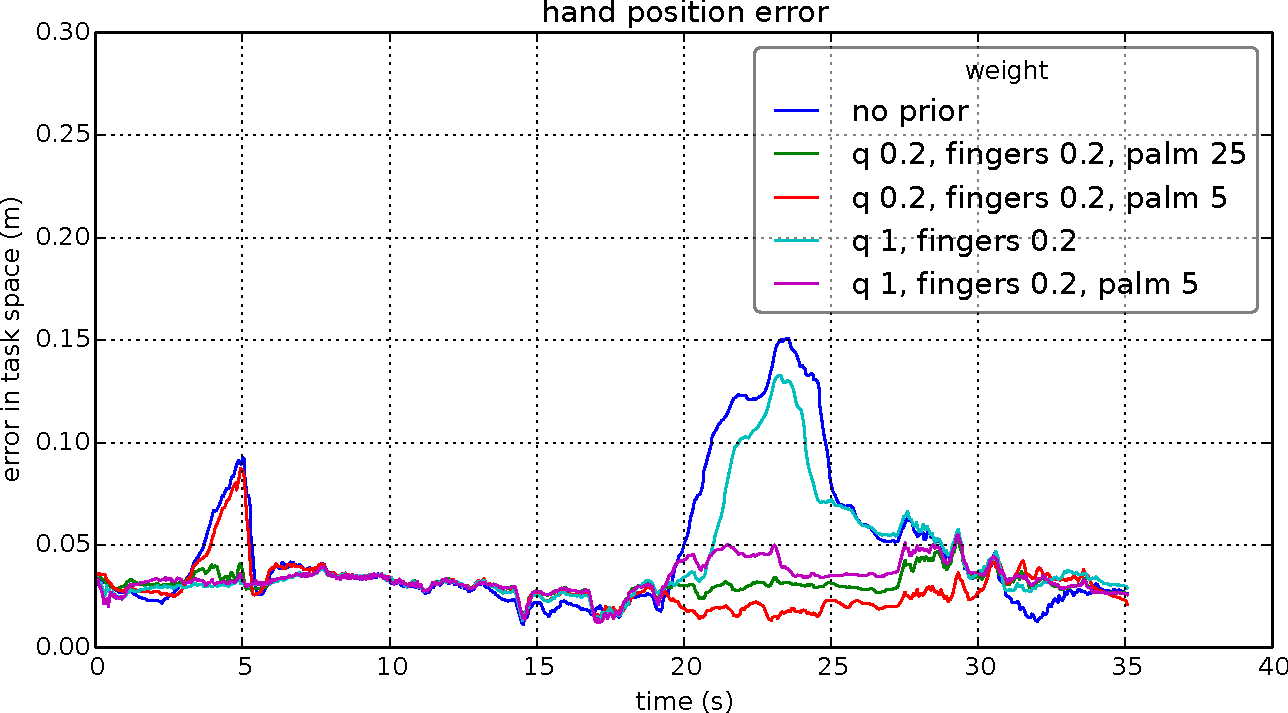
\includegraphics[width=0.5\textwidth]{images/eval_prior/inidv_weights/stereo_hand_pos_error.pdf} \label{fig:indiv_hand_pos_error}}
%
\subfloat[]{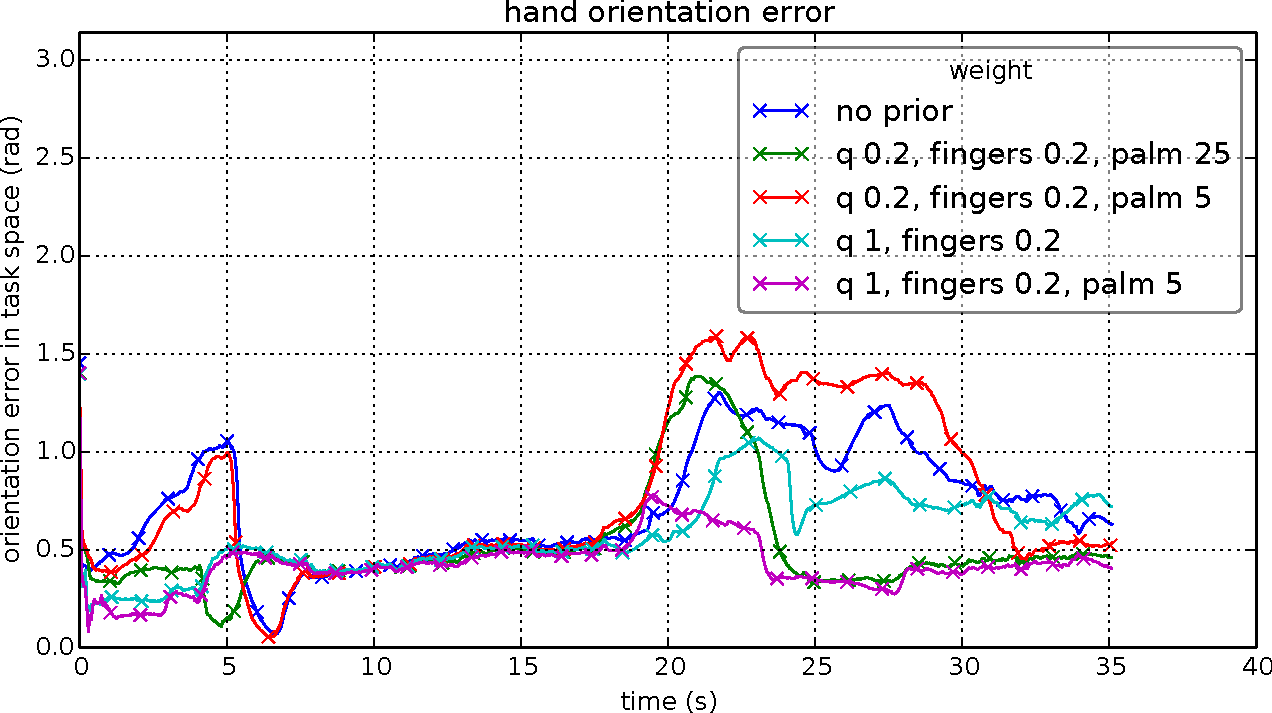
\includegraphics[width=0.5\textwidth]{images/eval_prior/inidv_weights/stereo_hand_ori_error.pdf} \label{fig:indiv_hand_ori_error}}

\caption{Task space error for individual weighting}
\label{fig:indiv_pose_error}
\end{figure}

\subsubsection{Object Position}

Most of the time, the pose of the object (bottle) is mainly affected by the optimization. Only when there is interaction between the manipulator and the object, it gets indirectly dependant on the joint values and hence the prior weight. The object's pose is initialise close to the true observed state and is expected to not move until the end of the reaching phase. Figure \ref{fig:bottle_movement} compares the object's distance to the image origin for stereo and xtion datasets and gives an indication about its movement. The bottle in the stereo data (figure \ref{fig:bottle_movement_stereo}) stays, as expected, close to its initial position until the end of the reaching phase. In contrast, the bottle in the Xtion dataset (figure \ref{fig:bottle_movement_xtion}) already moves at the beginning to its final pose.

\begin{figure}
\centering
\subfloat[stereo]{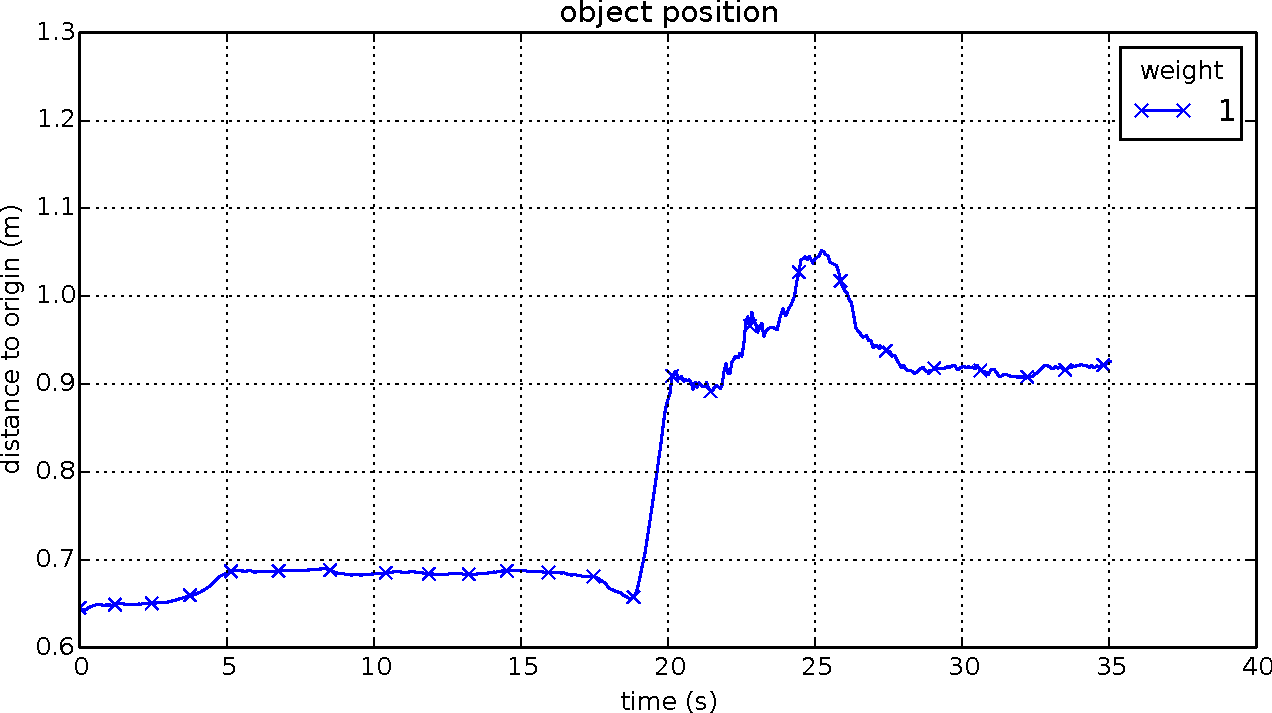
\includegraphics[width=0.5\textwidth]{images/eval_prior/stereo_obj_pos.pdf} \label{fig:bottle_movement_stereo}}
\subfloat[xtion]{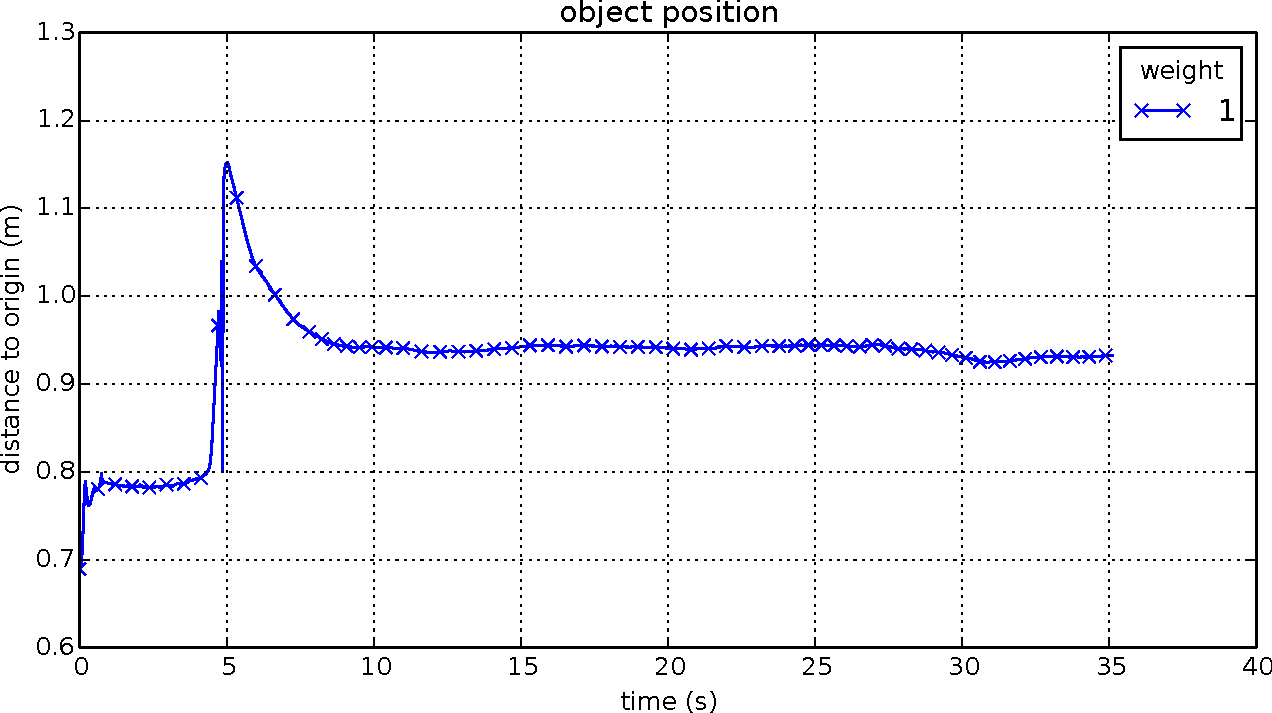
\includegraphics[width=0.5\textwidth]{images/eval_prior/xtion_obj_pos.pdf} \label{fig:bottle_movement_xtion}}
\caption{Movement of bottle during robot arm movement}
\label{fig:bottle_movement}
\end{figure}

A snapshot of the perceived point cloud is depicted in figure \ref{fig:bottle_point_cloud} for a state at the beginning of the experiment for both depth sources. A comparison of these sources show that: 1) the stereo depth source contains data with larger depth, and 2) the stereo depth source also contains more points of the object than the structured light sensor. It must be noted that the structured light sensor is mounted above the stereo sensor pointing into the same region of interest. It thus perceives the scene at a steeper angle.

\begin{figure}
\centering
\subfloat[stereo point cloud]{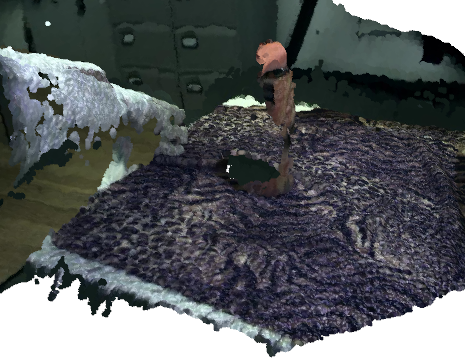
\includegraphics[width=0.4\textwidth]{images/eval_prior/stereo_bottle.png} }
\hspace{1cm}
\subfloat[xtion point cloud]{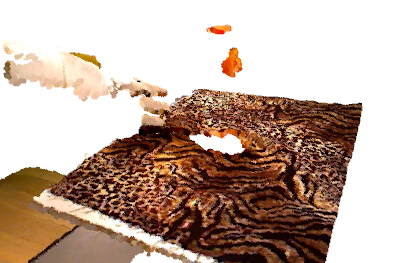
\includegraphics[width=0.4\textwidth]{images/eval_prior/xtion_bottle.png} }
\caption{Table and bottle in stereo and xtion point cloud}
\label{fig:bottle_point_cloud}
\end{figure}

\subsection{Interpretation}

\begin{itemize}
\item common joint weights are most beneficial for finger joints
\item individual weights are most beneficial for finger joints
\item high errors when distracting objects (table, bottle) are present, hence we find largest improvement in these cases
\item longer phase of oscillation for higher weights
\item Asus Xtion has smaller angle of view, e.g. objects having no associated points is more likely
\end{itemize}




\section{Filtered Manipulator Perception}

\subsection{Setup}

\begin{itemize}
\item data with moving arm and fingers
\item no distraction close to manipulator
\item ground truth vicon marker
\end{itemize}


\subsection{Hypotheses}

\begin{itemize}
\item no significant improvement by prior because of missing distraction
\item perceived hand pose closer to vicon state than reported state
\end{itemize}